\documentclass[tikz,border=10pt]{standalone}
\usepackage{amsmath}
\usetikzlibrary{arrows.meta, decorations.pathreplacing}

\begin{document}

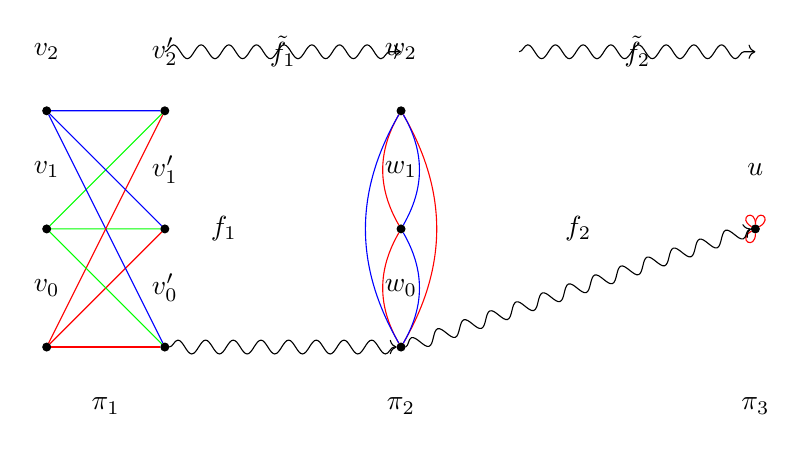
\begin{tikzpicture}[scale=1.5, every node/.style={circle, draw, fill=black, inner sep=1pt}]

    % First graph
    \node (v0) at (0,0) {};
    \node (v1) at (0,1) {};
    \node (v2) at (0,2) {};
    \node (v0') at (1,0) {};
    \node (v1') at (1,1) {};
    \node (v2') at (1,2) {};
    
    \draw[red] (v0) -- (v0');
    \draw[green] (v1) -- (v1');
    \draw[blue] (v2) -- (v2');
    \draw[red] (v0) -- (v1');
    \draw[green] (v1) -- (v2');
    \draw[blue] (v2) -- (v0');
    \draw[red] (v0) -- (v2');
    \draw[green] (v1) -- (v0');
    \draw[blue] (v2) -- (v1');

    \node[draw=none, fill=none] at (0.5,-0.5) {$\pi_1$};

    % Second graph
    \node (w0) at (3,0) {};
    \node (w1) at (3,1) {};
    \node (w2) at (3,2) {};
    
    \draw[red] (w0) to[bend left] (w1);
    \draw[red] (w1) to[bend left] (w2);
    \draw[red] (w2) to[bend left] (w0);
    \draw[blue] (w0) to[bend right] (w1);
    \draw[blue] (w1) to[bend right] (w2);
    \draw[blue] (w2) to[bend right] (w0);

    \node[draw=none, fill=none] at (3,-0.5) {$\pi_2$};

    % Third graph
    \node (u) at (6,1) {};
    
    \draw[red] (u) to[out=90, in=150, looseness=10] (u);
    \draw[red] (u) to[out=30, in=90, looseness=10] (u);
    \draw[red] (u) to[out=210, in=270, looseness=10] (u);

    \node[draw=none, fill=none] at (6,-0.5) {$\pi_3$};

    % Morphisms
    \node[draw=none, fill=none] (f1) at (1.5,1) {$f_1$};
    \node[draw=none, fill=none] (f2) at (4.5,1) {$f_2$};

    \draw[->, decorate, decoration={snake}] (v0'.east) -- (w0.west);
    \draw[->, decorate, decoration={snake}] (w0.east) -- (u.west);

    % Labels
    \node[draw=none, fill=none] at (0,2.5) {$v_2$};
    \node[draw=none, fill=none] at (0,1.5) {$v_1$};
    \node[draw=none, fill=none] at (0,0.5) {$v_0$};
    \node[draw=none, fill=none] at (1,2.5) {$v'_2$};
    \node[draw=none, fill=none] at (1,1.5) {$v'_1$};
    \node[draw=none, fill=none] at (1,0.5) {$v'_0$};

    \node[draw=none, fill=none] at (3,2.5) {$w_2$};
    \node[draw=none, fill=none] at (3,1.5) {$w_1$};
    \node[draw=none, fill=none] at (3,0.5) {$w_0$};

    \node[draw=none, fill=none] at (6,1.5) {$u$};

    \node[draw=none, fill=none] at (2,2.5) {$\tilde{f}_1$};
    \node[draw=none, fill=none] at (5,2.5) {$\tilde{f}_2$};

    \draw[->, decorate, decoration={snake}] (1,2.5) -- (3,2.5);
    \draw[->, decorate, decoration={snake}] (4,2.5) -- (6,2.5);

\end{tikzpicture}

\end{document}